\chapter{Hitting set}
\label{ch:hittingset}
\index{hitting set problem}

Chapters~\ref{ch:potts}--\ref{ch:ising} carried one number per inclusion all the
way from $q=1$ to $q=\infty$. This chapter is where that stops.
The failure it identifies, and the repair, are new here; the closed forms it
reproduces at cardinality two are those of \citet{weigt2000} and
\citet{mezard2007}, and are attributed at each use.

The problem is a hard-core one: minimise a set subject to a constraint that some
configurations are simply forbidden. Nothing in Chapter~\ref{ch:statmech}
objects --- Eq.~\eqref{eq:emitted} sums whatever is inside a complex, and an
infinite energy is a legitimate thing to put there. What changes is that the
standard way of taking the zero-temperature limit, which is exact on a graph and
has been used on graphs for twenty-five years, is \emph{wrong} on a hypergraph.
Section~\ref{sec:hardfail} gives a counterexample small enough to check by hand,
and Sec.~\ref{sec:soft} gives the repair.

The failure is this chapter's version of something the book keeps returning to.
It is not that the cavity method fails on higher-order structures. It is that a
simplification which is invisible on a graph, because it costs nothing there,
becomes the whole error once complexes hold more than two nodes.

\section{Covering a family of sets}
\label{sec:hittingsetdef}

A \emph{hitting set} meets every hyperedge: a set of nodes such that no
hyperedge is left entirely outside it. Minimising it generalises vertex cover
from graphs to hypergraphs \citep{mezard2007}. Put $x_{i}=1$ when node $i$ is in
the set and $x_{i}=0$ when it is not, and write
\begin{equation}
  \mathcal{H}=\mu\sum_{i}x_{i}
  \qquad\text{subject to}\qquad
  \prod_{e}\Bigl[1-\prod_{i\in e}(1-x_{i})\Bigr]=1,
  \label{eq:Hhs}
\end{equation}
the constraint forbidding a hyperedge none of whose members is taken, and the
chemical potential $\mu$ penalising every member, so that minimum hitting sets
are the ground states reached as $\mu\to\infty$.

At cardinality two this is minimum vertex cover, Sec.~\ref{sec:cover-intro}, and
Chapter~\ref{ch:cover} is what happens when the constraint is tightened instead
of the cardinality raised. The two problems sit at opposite ends of one family
and differ in one line of the interior sum. The failure this chapter is about is
invisible at cardinality two, which is where the literature works.

It is often convenient to work with the complement $y_{i}=1-x_{i}$, which is a
\emph{packing} --- no hyperedge lies wholly inside it --- since the hard-field
limit is naturally written that way, the cover being one minus the packing
density.

\section{Hard fields}
\label{sec:hard}
\index{hard field|textbf}
\index{warning propagation|textbf}

The standard treatment rescales the cavity fields, which diverge as
$\mu\to\infty$: put $h=\mu z$ and keep only the integer $z$. The up step of
Eq.~\eqref{eq:up} becomes a count,
\begin{equation}
  z_{i}=1-\#\bigl\{\,b\ni i:\ z_{j\to b}=1\ \ \forall\,j\in b\setminus i\,\bigr\},
  \label{eq:zhs}
\end{equation}
which is \emph{warning propagation}: a complex sends a warning when every one of
its other members is free to stay out, and a node counts its warnings.

Two steps take that to an ensemble. Let $\sigma_{l}$ be the probability that a
node reached along an inclusion into a layer-$l$ complex has $z=1$, that is, is
free to stay out. A layer-$l$ complex entered at $i$ warns $i$ exactly when
every one of its other $c_{l}-1$ members is free, and on a treelike chygraph
those members are independent given what reaches them, so
$\tau_{l}=\sigma_{l}^{\,c_{l}-1}$. And $i$ is free precisely when \emph{none} of
its other complexes warns it; each fails to warn with probability $1-\tau$, how
many others there are is the excess chy-degree of Sec.~\ref{sec:ensembles}, and
averaging a product over that count is evaluating its generating function. So
\begin{equation}
  \sigma_{m}=\bar\Phi^{(m)}(1-\tau),
  \qquad
  \tau_{l}=\sigma_{l}^{\,c_{l}-1}.
  \label{eq:hs}
\end{equation}
Section~\ref{sec:twoconstraints} does the same two steps for vertex cover and
gets the complement in the other place, for the reason given there: a hyperedge
forces when \emph{all} of its other members are free and a clique forces when
\emph{any} of them is. \code{hittingset.HittingSet.F} is the map and
\code{hittingset.HittingSet.solve} its fixed point.

\paragraph{The map runs backwards.} Equation~\eqref{eq:hs} is
order-\emph{reversing}: raising any message lowers every message. This is not a
technicality. Plain iteration oscillates, and past the point where the map loses
stability it never settles --- which is how the instability was originally
detected \citep{vazquez2003vw}, by noticing that the program stopped converging.
It is also the diagnostic Sec.~\ref{sec:fixedpoint} said would be needed, and
the reason it insisted on reading the \emph{signs of the entries} rather than
the sign of the leading eigenvalue.

It need not be left to chance. For $F$ continuous and order-reversing on
$[0,1]^{L}$ --- both hold here, since $\bar\Phi$ is a power series with
non-negative coefficients and $\sigma\mapsto1-\sigma^{c-1}$ is decreasing ---
the composition $F\circ F$ is order-\emph{preserving}. Iterating $F\circ F$ from
$0$ and from $1$ therefore returns its least and greatest fixed points $a\le b$
with $F(a)=b$. If $a=b$ there is a single stable fixed point; if $a<b$ there is
a period-two orbit with the fixed point of $F$ strictly between them, unstable.
The bracket finds the solution and diagnoses it in one pass, which is a better
bargain than watching an iteration fail to converge.

\paragraph{Where it loses stability.} At fixed cardinality $c$ with Poisson
chy-degree, $\bar\Phi(x)=e^{\ave{k}(x-1)}$ and Eq.~\eqref{eq:hs} closes on one
scalar.

With one layer and Poisson chy-degree the map is
$\sigma=e^{-\ave{k}\sigma^{c-1}}$. Differentiating and using the fixed-point
relation,
\[
  |F'(\sigma)|=\ave{k}(c-1)\sigma^{c-2}e^{-\ave{k}\sigma^{c-1}}
             =\ave{k}(c-1)\sigma^{c-1}.
\]
Put $y=\ave{k}\sigma^{c-1}$. The fixed point reads $\sigma=e^{-y}$ and
$y=\ave{k}e^{-(c-1)y}$, while the instability $|F'|=1$ is $(c-1)y=1$.
Eliminating $y=1/(c-1)$ from the second,
\[
  \ave{k}=y\,e^{(c-1)y}=\frac{e}{c-1},
  \qquad\text{that is}\qquad
  \ave{k}\,(c-1)=e.
\] \code{hittingset.\allowbreak rsb\_\allowbreak point} solves it, and returns $e$ at $c=2$ to ten digits.

So
\begin{equation}
  \ave{k}\,(c-1)=e,
  \label{eq:kc}
\end{equation}
verified to eleven digits for $c=2,\dots,20$. Read in \emph{neighbours} per
node, cardinality does not move the point at all: a hyperedge of size six
supplies five neighbours and costs a fifth of the chy-degree, and the two cancel
exactly. At $c=2$ this returns $\ave{k}=e$, the Bauer--Golinelli value
\citep{bauer2001}, which Chapter~\ref{ch:cover} will show is three quantities
with one name.

\paragraph{What Eq.~\eqref{eq:kc} is a statement about.} It locates the loss of
stability of the \emph{hard-field} map --- which is to say, where
leaf-removal-style certification stops. At $c=2$ that coincides with the
accepted replica-symmetry-breaking point, which is why $e$ comes out. Above
$c=2$ it does not, and the next section is why.

\section{Where the hard-field limit breaks}
\label{sec:hardfail}
\index{hard field}

Equation~\eqref{eq:zhs} discards an $O(1)$ contribution: it keeps the part of
$h$ proportional to $\mu$ and throws away the remainder. On a graph the discard
is harmless. On a hypergraph it is the answer.

The cleanest demonstration needs no computer. Take disjoint $3$-hyperedges, one
per vertex --- so every vertex belongs to exactly one hyperedge and no two
hyperedges touch (Fig.~\ref{fig:counterexample}). There is no interaction
between complexes at all. Replica symmetry is trivially valid, there is nothing
for it to break. One of every three vertices must be taken, so the minimum
hitting set has density exactly $1/3$.

The hard-field calculation returns $1/2$.

\begin{figure}[t]
\centering
\begin{adjustbox}{max width=0.95\linewidth}
\begin{tikzpicture}
% Three disjoint 3-hyperedges. Nothing couples them, so replica symmetry is
% trivially valid and the answer is exactly 1/3 -- which is what makes this a
% counterexample rather than a hard case.
\foreach \s in {0,1,2}{
  \begin{scope}[xshift=\s*2.35cm]
    \node[nd] (a\s) at (-0.55,0) {};
    \node[hub] (b\s) at (0.0,0.46) {};
    \node[nd] (c\s) at (0.55,0) {};
    \draw[lnk] (a\s)--(b\s)--(c\s)--(a\s);
    \begin{scope}[on background layer]
      \node[cx,fit=(a\s)(b\s)(c\s)] {};
    \end{scope}
  \end{scope}
}
\node[lb,anchor=north,align=center] at (2.35,-0.62)
  {the dark vertex of each triple is taken: density $1/3$};
\node[lb,anchor=west,align=left] at (5.85,0.20)
  {hard fields: $0.5$\\ soft fields: $0.3333$};
\end{tikzpicture}
\end{adjustbox}
\caption{\textbf{A counterexample that fits on one line.} Disjoint
$3$-hyperedges, one per vertex. No complex touches another, so the cavity
equations are exact and replica symmetry cannot break. One vertex per hyperedge
must be taken and the density is exactly $1/3$. The hard-field limit,
Eq.~\eqref{eq:zhs}, returns $1/2$ --- and its bracket is the whole interval
$(0,1)$, so it cannot even report that it is in trouble. Keeping the $O(1)$
fields, Eq.~\eqref{eq:soft}, returns $1/3$.}
\label{fig:counterexample}
\end{figure}

The mechanism is precise. Inside such a hyperedge every vertex sits at $z=0$: the
integer message cannot distinguish the taken vertex from the two left out,
because the distinction is carried by the $O(1)$ part that was scaled away. A
vertex at $z=0$ is degenerate, and the standard rule counts it as half covered
--- which is right when the degeneracy is two-fold, as it is on a graph, and
wrong when it is three-fold. The bracket of Sec.~\ref{sec:hard} returns $(0,1)$
here, so the hard-field scheme cannot even report that it is in difficulty.

The second failure follows from the first. Equation~\eqref{eq:kc} is a property
of the hard-field map and not of the full replica-symmetric solution, and the
two coincide only at cardinality two. On random regular hypergraphs the
hard-field criterion reports broken symmetry across almost the whole grid where
\citet{mezard2007} find a genuine replica-symmetric region --- though it
does reproduce their result that cardinality two breaks at every degree.

\section{Keeping the fields}
\label{sec:soft}
\index{soft field|textbf}
\index{population dynamics}

Both failures are repaired by not scaling the fields at all.

Work directly with Eq.~\eqref{eq:Hhs}: $x_{i}=1$ for a vertex in the set, weight
$e^{-\mu\sum_{i}x_{i}}$, no change of variable. Belief propagation on the
chygraph then reads
\begin{align}
  v_{a\to i}&=-\ln\Bigl[1-\prod_{j\in a\setminus i}
                \bigl(1+e^{h_{j\to a}}\bigr)^{-1}\Bigr],\nonumber\\
  h_{i\to a}&=-\mu+\sum_{b\ni i,\ b\ne a}v_{b\to i},
  \label{eq:soft}
\end{align}
with the density read off the full field,
$\rho=\bigl[1+e^{\,\mu-\sum_{b\ni i}v_{b\to i}}\bigr]^{-1}$.

These are Chapter~\ref{ch:statmech}'s two steps and nothing else. The chy-degree
step is the convolution of Sec.~\ref{sec:upstep}; the complex step is the sum
over the interior of Sec.~\ref{sec:downstep}, here over the single forbidden
configuration in which no member is taken. What has changed against
Sec.~\ref{sec:hard} is only that nothing is divided by $\mu$, so the $O(1)$
parts survive and $\rho$ emerges as a genuine $O(1)$ number rather than a count
of integers.

For a regular hypergraph --- $L$ complexes per node, each of cardinality $K$ ---
symmetry makes every message equal and Eq.~\eqref{eq:soft} closes on a pair:
\[
  h=-\mu+(L-1)v,
  \qquad
  v=-\ln\Bigl[1-\bigl(1+e^{h}\bigr)^{-(K-1)}\Bigr].
\]
As $\mu\to\infty$, $h\to-\infty$ and
$(1+e^{h})^{-(K-1)}=1-(K-1)e^{h}+O(e^{2h})$, so the complex step becomes
$v=-\ln(K-1)-h$. Substituting, $Lh=-\mu-(L-1)\ln(K-1)$, that is
\begin{equation}
  h_{\mathrm{RS}}=-\frac{\mu}{L}-\frac{L-1}{L}\ln(K-1).
  \label{eq:hRS}
\end{equation}
The cavity field carries a \emph{fraction} $1/L$ of $\mu$. An ansatz restricted to integer multiples of $\mu$ cannot represent it,
and that --- not any subtlety about correlations --- is why
Sec.~\ref{sec:hardfail} fails.

The full field is finite, $H=h+v=-\ln(K-1)$, so
\[
  \rho=\frac{1}{1+e^{-H}}=\frac1K,
\]
independent of $\mu$ \emph{and} of $L$: one member of every complex is taken and
none is wasted, so the counting bound is saturated exactly. \code{softfield.\allowbreak regular\_\allowbreak field} is the closed form,
and the population dynamics it is checked against is
\code{Chygraph.\allowbreak hitting\_\allowbreak set\_\allowbreak bp}, over
\code{softfield.\allowbreak HittingSetBP}.

Equation~\eqref{eq:hRS} and $\rho=1/K$ are the closed forms of
\citet{mezard2007}, and population dynamics reproduces both --- the field
to five decimals, the density to four. The repair is complete on the
counterexample too: disjoint $3$-hyperedges return $0.3333$.
Figure~\ref{fig:hitting} runs the comparison across ensembles.

\begin{figure}[t]
\centering
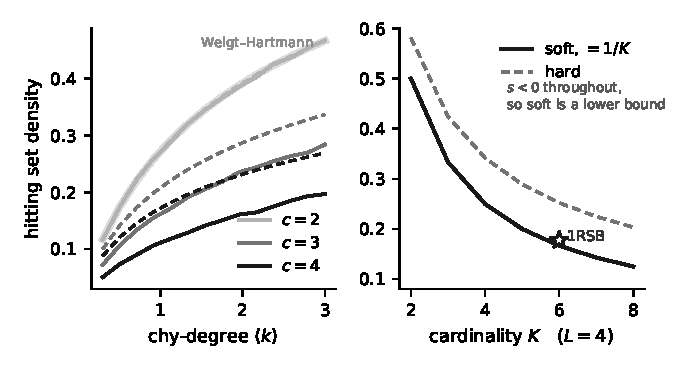
\includegraphics[width=\linewidth]{figs/fig-hitting.pdf}
\caption{\textbf{The repair.} Minimum hitting-set density from the hard-field
limit, Eq.~\eqref{eq:hs} with the half rule (dashed), and from
Eq.~\eqref{eq:soft}, which keeps the $O(1)$ fields (solid). Left: Poisson
layers of one cardinality, with the Weigt--Hartmann closed form drawn thick
behind the $c=2$ curves, which the two treatments share exactly. They separate
above cardinality two and the gap grows with $c$. Right: regular hypergraphs at
$L=4$. The soft field returns $\rho=1/K$; the hard field does not; and at $K=6$
the two bracket the one-step replica-symmetry-breaking value of
\citet{mezard2007} (star), $0.1667<0.178<0.2522$. Generated by
\code{figs/\allowbreak hittingset.\allowbreak py}.}
\label{fig:hitting}
\end{figure}

At cardinality two hard and soft \emph{must} agree, and do: both return the
Weigt--Hartmann cover size $1-(2W+W^{2})/(2\ave{k})$ with
$W=\mathcal{W}(\ave{k})$, the hard field to six digits and the soft field to
within its sampling scatter of a few parts in a thousand. Above cardinality two
the correction grows with the weight the ensemble puts on complexes of three or
more members: for a Poisson layer of $c=4$ alone at $\ave{k}=1$ the hard field
overstates the density by about $55$ per cent, $0.172$ against $0.111$, and for
a mixture of $c=2$ and $c=6$ at chy-degrees $1.5$ and $0.5$ by under one per
cent. That last number is the reassuring one: it says the twenty-five years
of graph results were never in danger.

\section{What the chygraph structure adds}
\label{sec:hsstructures}

Equation~\eqref{eq:soft} carries an arbitrary chy-degree distribution, mixed
cardinalities and correlated layers, none of which a regular ansatz reaches.
Two effects, pointing in opposite directions.

\emph{Spread in cardinality postpones the difficulty.} Hold fixed the mean
number of neighbours a complex supplies, $\nu=\sum_{l}\ave{k_{l}}(c_{l}-1)
/\sum_{l}\ave{k_{l}}$, at $2$, and report $\ave{k}\nu$, the neighbours per node
at which Eq.~\eqref{eq:kc}'s instability arrives. It runs from $2.72$ for
uniform $c=3$, to $4.84$ for an equal mixture of $c=2$ and $c=4$, to $6.83$ for
a three-to-one mixture of $c=2$ and $c=6$. Heterogeneity keeps certification
working longer, which is the direction degree heterogeneity acts in as well
\citep{vazquez2003vw}.

\emph{Correlation across cardinalities brings it forward.} Anti-correlate a
node's participation in small and in large hyperedges, holding the marginals
fixed, and the point moves monotonically down from $6.83$ to $2.64$. This axis has no counterpart
in an ensemble with one edge type, and it is the sort of thing
Chapter~\ref{ch:data} recommended measuring rather than assuming away.

\paragraph{A confound.} The obvious positive-correlation
construction --- half the nodes at double the chy-degree, half at zero ---
returns a point at exactly half the uncorrelated value, and that is not
correlation but \emph{dilution}: the zero class is a set of isolated vertices.
Matched constructions keep both classes populated, and $\Phi(0,\dots,0)$, the
fraction of vertices in no hyperedge at all, should be reported alongside any
such comparison. On the positive branch it rises from $0.033$ to $0.47$ as the
correlation is pushed to its extreme, so only its small-spread end is a clean
measurement. The negative branch is cleaner but not innocent. Neither class ever
empties there, since anti-correlation moves chy-degree between the layers rather
than out of both at once; but the ensemble is sparser at its own threshold, and
$\Phi(0,\dots,0)$ still runs $0.033$, $0.047$, $0.198$, $0.321$ across the four
spreads. The direction is settled at the second of those, where dilution is
negligible and the point has already moved from $6.83$ to $6.50$. The size of
the full excursion to $2.64$ is not separable from the dilution that comes with
it, and is not quoted as though it were.

\section{When replica symmetry fails}
\label{sec:hsrsb}
\index{replica symmetry breaking}

Section~\ref{sec:replicas} listed three signals. This chapter can now supply the
second, and it is the one that carries a number.

The Bethe free energy of Sec.~\ref{sec:freeenergy} applies unchanged, with
$Z_{i}=1+e^{H_{i}}$ and $Z_{a}=\prod_{i\in a}(1+e^{h_{i\to a}})-1$ --- the
complex term being the sum over its interior with the one forbidden
configuration removed --- so that
\begin{equation}
  s=\sum_{l}n_{l}\ave{\ln Z_{a}}+\ave{(1-k)\ln Z_{i}}+\mu\rho.
  \label{eq:sgen}
\end{equation}
For a regular hypergraph this reduces to
\begin{equation}
  s=\frac{1}{K}\bigl[a\ln(K-1)-(a-1)\ln K\bigr],
  \qquad
  a=(L-1)(K-1),
  \label{eq:entropy}
\end{equation}
which is \citeauthor{mezard2007}'s expression, reproduced by
Eq.~\eqref{eq:sgen} to nine digits. Since $s$ is the logarithm of a number of
ground states, a negative value counts fewer than one configuration, which is
impossible: where $s<0$ the replica-symmetric answer is wrong and is an
\emph{underestimate}. At $L=4$, $K=6$ the entropy is $-0.157$, and indeed the
replica-symmetric $1/6$ sits below the one-step $0.178$ while the hard-field
$0.252$ sits above it and further away.

Three qualifications, and all three matter in practice.

\emph{It is sufficient but not necessary.} A negative $s$ proves the answer
wrong; a positive $s$ does not prove it right, since a solution can be unstable
while its entropy is still positive. Vertex cover on Poisson graphs is the
standing example: replica symmetry breaks at $\ave{k}=e$, and yet
Eq.~\eqref{eq:sgen} returns $s=+0.088(26)$ at $\ave{k}=1$ and a value still
positive at $3$. The entropy has to be paired with a stability criterion, not
used alone.

\emph{It is not numerically cheap.} In Eq.~\eqref{eq:sgen} the terms
$\sum_{l}n_{l}\ave{\ln Z_{a}}$ and $\mu\rho$ are each $O(\mu)$ while $s$ is
$O(1)$, so a heterogeneous ensemble needs both to a relative precision of order
$s/\mu$ and only time-averaging the estimator brings that within reach. The
regular case is exact because symmetry removes the sampling entirely --- the two
$O(\mu)$ pieces cancel algebraically rather than statistically.

\emph{The third signal still shows up.} At $L=6$, $K=12$ the closed-form entropy
is $-0.192$ and the iteration simply does not settle; the estimator returns a
small positive number that means nothing. That is Sec.~\ref{sec:replicas}'s
third signal --- the equations stop converging --- and it is the same failure
the negative entropy reports, arriving by a different route.

What one-step replica symmetry breaking would change here, this book does not
compute. Sections~\ref{sec:colouring-sp} and~\ref{sec:sat-sp} do the one-step
calculation for two problems whose messages are warnings, where a survey is a
distribution over a finite alphabet; a hitting-set field is a real number and
the survey is a distribution over distributions, which is a heavier object and
is not attempted. What this chapter can say is where the replica-symmetric
answer stops being trustworthy, and on which side of the truth it then falls.

\section{Checks}
\label{sec:hs-checks}

\checkhead{Known results}
At cardinality two both treatments return the Weigt--Hartmann cover size, the
hard field to six digits, and Eq.~\eqref{eq:kc} returns $e$ there, which is
Bauer--Golinelli. Equations~\eqref{eq:hRS} and~\eqref{eq:entropy} reproduce
\citeauthor{mezard2007}'s closed forms, the first to five decimals by population
dynamics and the second to nine digits by Eq.~\eqref{eq:sgen}.

\checkhead{New results}
Everything above cardinality two is new here: the failure of the hard-field
limit, the repair, and Eq.~\eqref{eq:kc} away from $c=2$, which is verified to
eleven digits for $c=2,\dots,20$. The failure is checked against arithmetic
rather than against the literature. Section~\ref{sec:hardfail}'s counterexample
is not a numerical check but a proof: the answer is $1/3$ by counting, the soft
field returns $0.3333$, and the hard field returns $0.5$. Nothing about it
depends on an implementation being right.

\checkhead{Partial results}
Soft-field densities on Poisson ensembles come from a population of finite size
and carry a scatter of a few parts in a thousand that does not shrink cleanly
with the population; they are quoted to three decimals with the spread across
seeds beside them, and the regular cases carry no such scatter. The entropy of
Eq.~\eqref{eq:sgen} is sufficient and not necessary: a negative value proves the
replica-symmetric answer wrong, a positive one proves nothing, and vertex cover
on Poisson graphs is the standing example. What replica symmetry breaking would
change is not computed --- a hitting-set field is a real number, so the survey is
a distribution over distributions, and Sec.~\ref{sec:hsrsb} states the cost and
stops there.
